\documentclass[a4paper]{article}

\usepackage{fullpage} % Package to use full page
\usepackage{parskip} % Package to tweak paragraph skipping
\usepackage{tikz} % Package for drawing
\usepackage{amsmath}
\usepackage{hyperref}
\usepackage{subcaption}
\usepackage{graphicx}
\usepackage{fancyvrb}

\title{16-720B Computer Vision: Homework 1 \\
Spatial Pyramid Matching for Scene Classification}
\author{Heethesh Vhavle\\
Andrew ID: hvhavlen}
\date{24 September 2018}

\begin{document}

\maketitle

\section{Representing the World with Visual Words}
\subsection{Extracting Filter Responses}
\subsubsection{Answer}

The filters used can grouped into three categories as follows:
\begin{itemize}
    \item Gaussian Filter - This is a low pass filter which is effective in reducing noise in images. Since images will have noise in them and we would like to pick good features, we use Gaussian filters to get noiseless features. It is better than other averaging filters such as Mean or Median as it has weighted responses and gives more weight to the center pixels so that not much of spatial information is lost. It has similarities with the human perception system and has been found that neurons create a similar filter when processing images. 
    \item Laplacian of Gaussian Filter - This is a second derivative filter which gives zero response for uniform regions in an image and positive/negative response in regions where there are changes. These filters are commonly used to detect blob-like features in images. The Laplacian filter is usually applied after a Gaussian filter to smooth it and improve the response, as derivative filters are highly sensitive to noise.
    \item First Derivative Filters - These filters are applied in the X and Y directions separately, and are used to detect vertical and horizontal edge-like features respectively. Again, these filters are applied after a Gaussian filter to smooth it and improve the response, as derivative filters are highly sensitive to noise.
\end{itemize}

We need multiple scales of the above filters because the size of features vary in different images, and we would like our filter bank to pick all these multi-sized features. For example, to detect an edge which is far away from the camera, we may need a smaller filter, and to detect edges associated with buildings and other large objects, we require filters with larger kernels. Hence we vary the size of kernels by changing the sigma value.

\subsubsection{Filter Responses}
The 20 extracted filter responses are shown in Figure \ref{filterresponses}.

\begin{figure}[!htbp]
\begin{center}
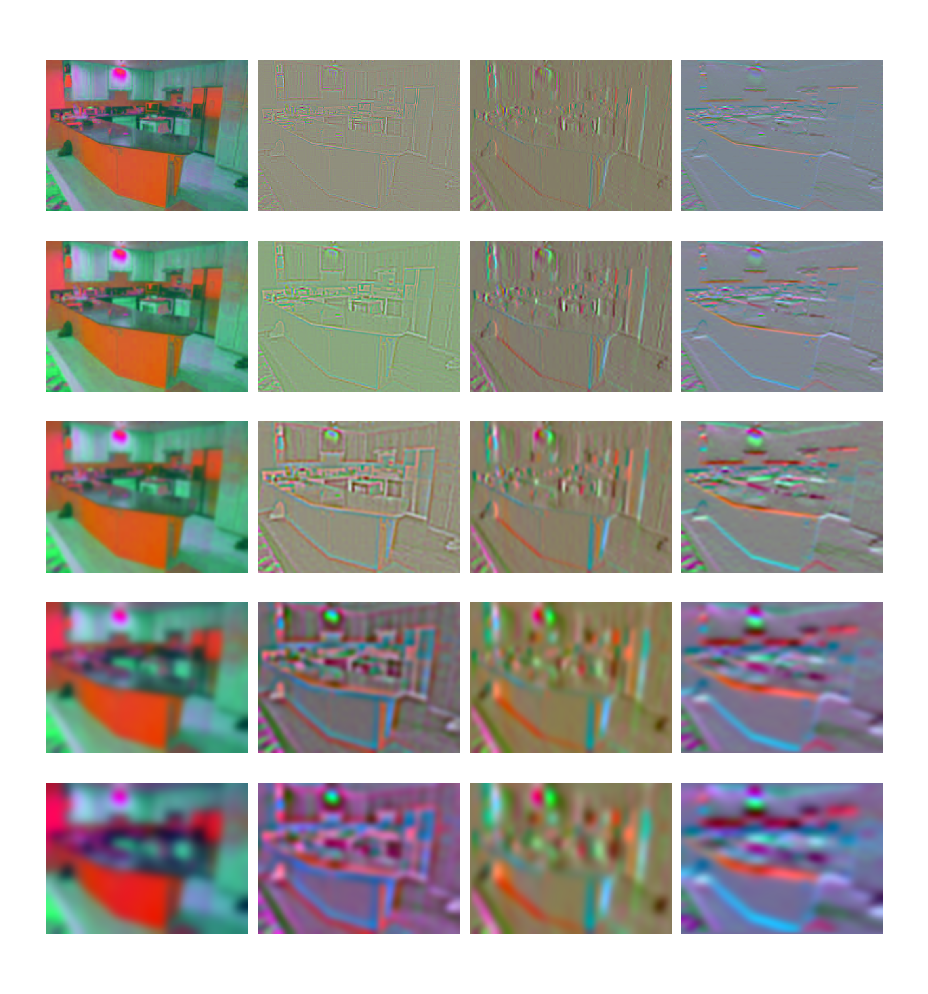
\includegraphics[scale=0.6]{filter_responses2.png}
\end{center}
\caption{The extracted filter responses.}\label{filterresponses}
\end{figure}

\newpage

\subsection{Creating Visual Words}
The \textit{dictionary.npy} file has been created with the following parameters.

\begin{equation*}
\begin{aligned}
    \alpha = 150\\
    K = 100
\end{aligned}
\end{equation*}

\subsection{Computing Visual Words}
The wordmaps have been generated using the dictionary and are visualized below. It can be observed that some of the features such as the seats in the auditorium have been assigned the same word (colored in pink). Some classes have images rich in features and lot of variations like \textit{laundromat} and \textit{windmill}, and have more visual words. The \textit{desert} class, with almost uniform regions has very few visual words.

\begin{figure}[!ht]
\centering
\begin{tabular}{ccc}
{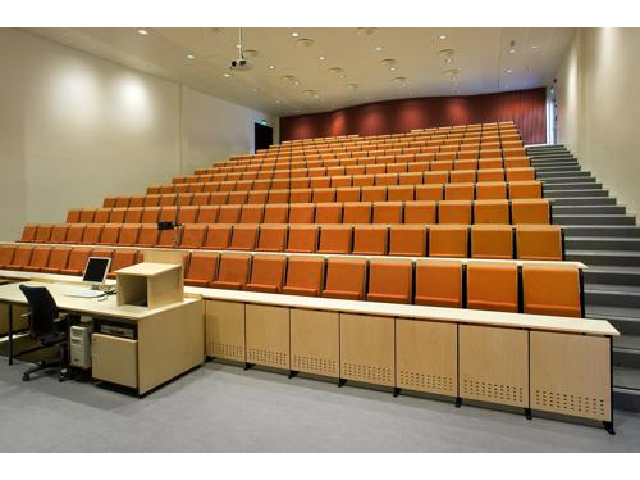
\includegraphics[width=0.3\textwidth]{auditorium}} &
{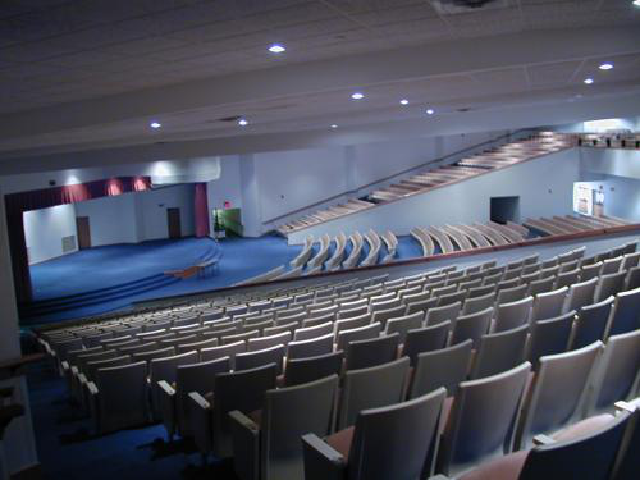
\includegraphics[width=0.3\textwidth]{audi2}} &
{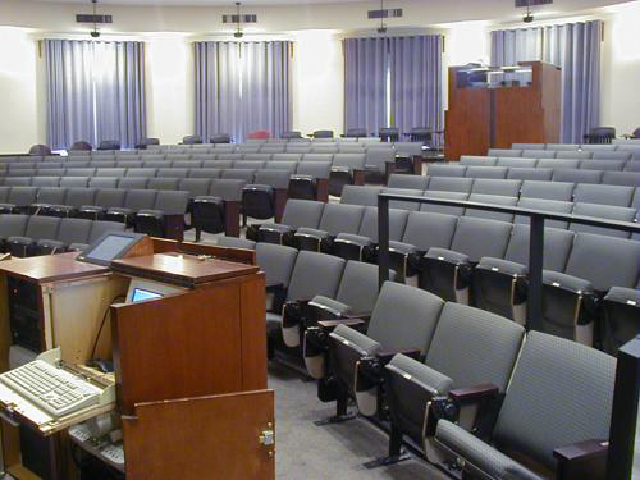
\includegraphics[width=0.3\textwidth]{audi3}} \\
{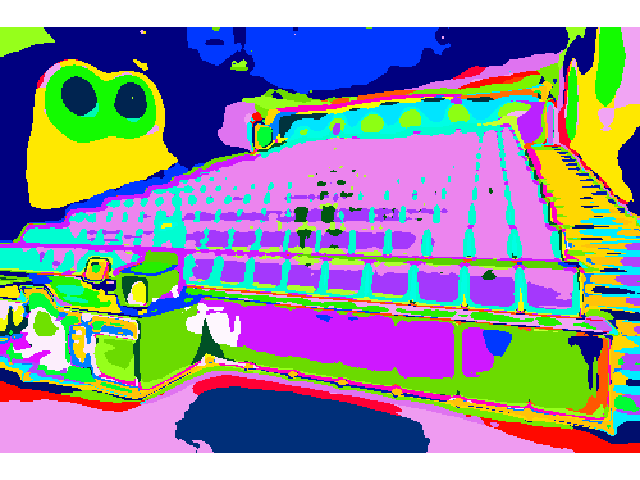
\includegraphics[width=0.3\textwidth]{auditorium_wordmap}} &
{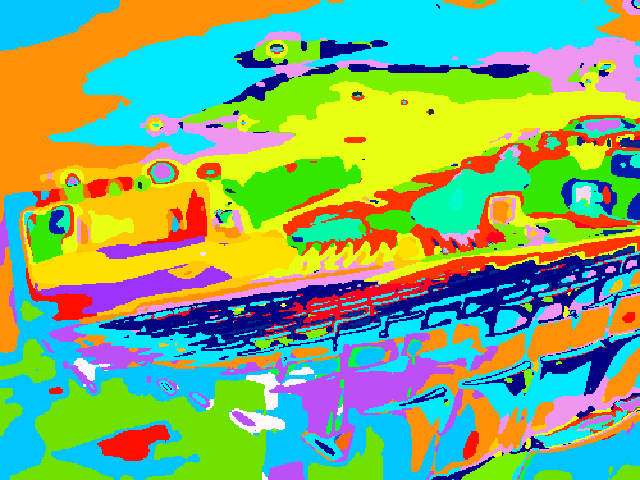
\includegraphics[width=0.3\textwidth]{audi2_wordmap}} &
{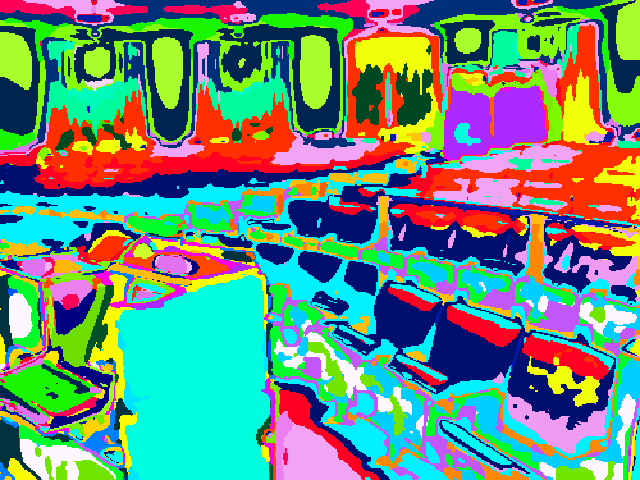
\includegraphics[width=0.3\textwidth]{audi3_wordmap}}\\
\end{tabular}
\caption{Three different images of the auditorium class are visualized with their wordmaps.}
\end{figure}

\begin{figure}[!ht]
\centering
\begin{tabular}{ccc}
{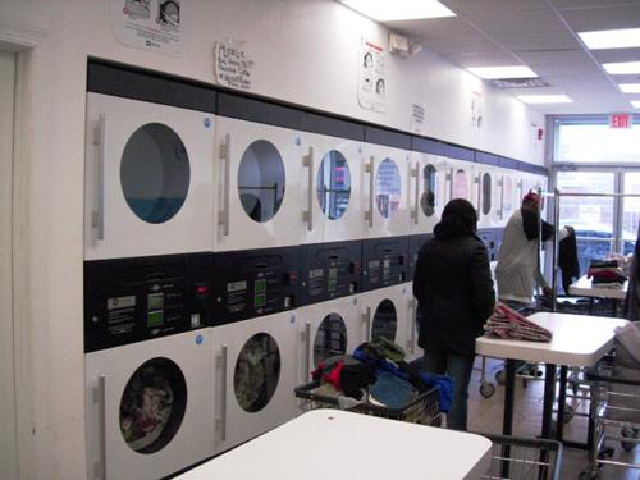
\includegraphics[width=0.3\textwidth]{laundromat}} &
{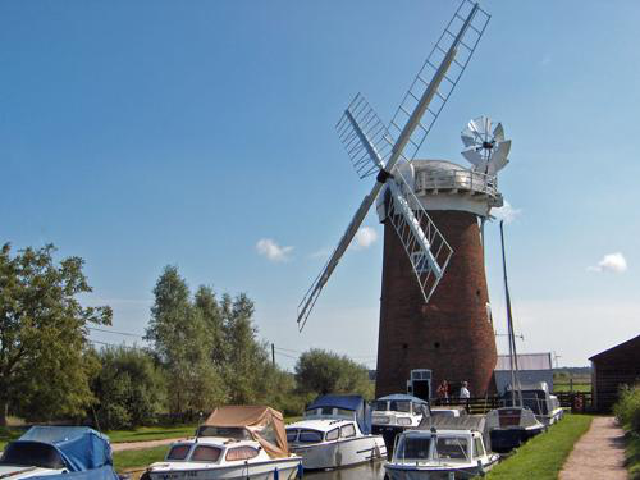
\includegraphics[width=0.3\textwidth]{windmill}} &
{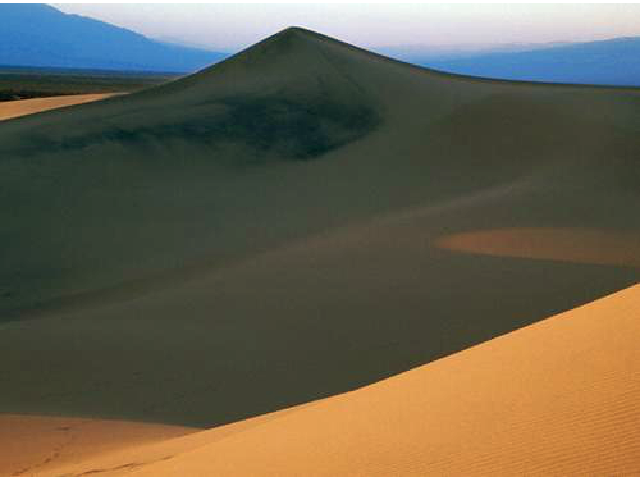
\includegraphics[width=0.3\textwidth]{desert}} \\
{
\includegraphics[width=0.3\textwidth]{laundromat_wordmap}} &
{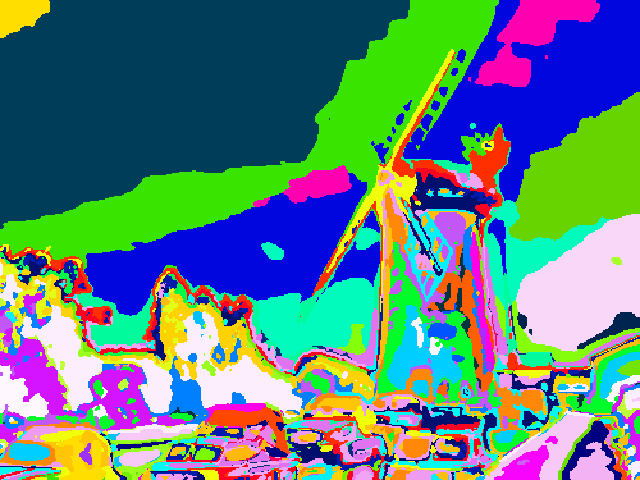
\includegraphics[width=0.3\textwidth]{windmill_wordmap}} &
{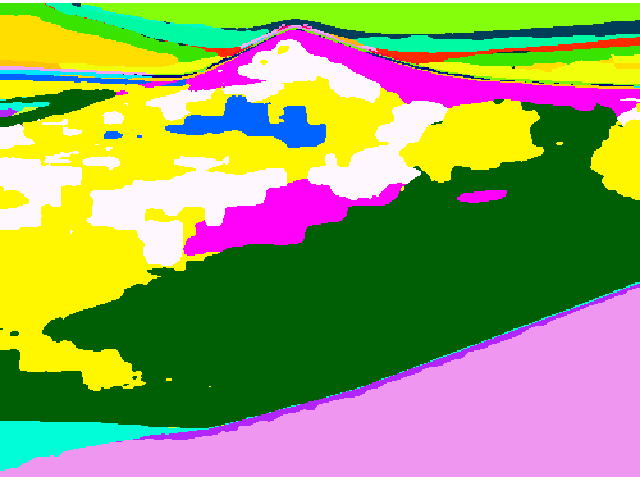
\includegraphics[width=0.3\textwidth]{desert_wordmap}} \\
\end{tabular}
\caption{Images from laundromat, windmill, and desert classes are visualized with their wordmaps.}
\end{figure}

\section{Building a Recognition System}
\subsection{Extracting Features}

\begin{figure}[!ht]
\centering
\begin{tabular}{c}
{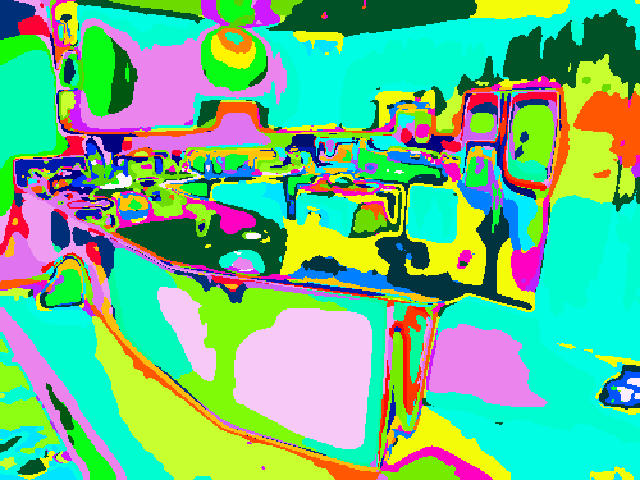
\includegraphics[width=0.9\textwidth]{kitchen}} &
{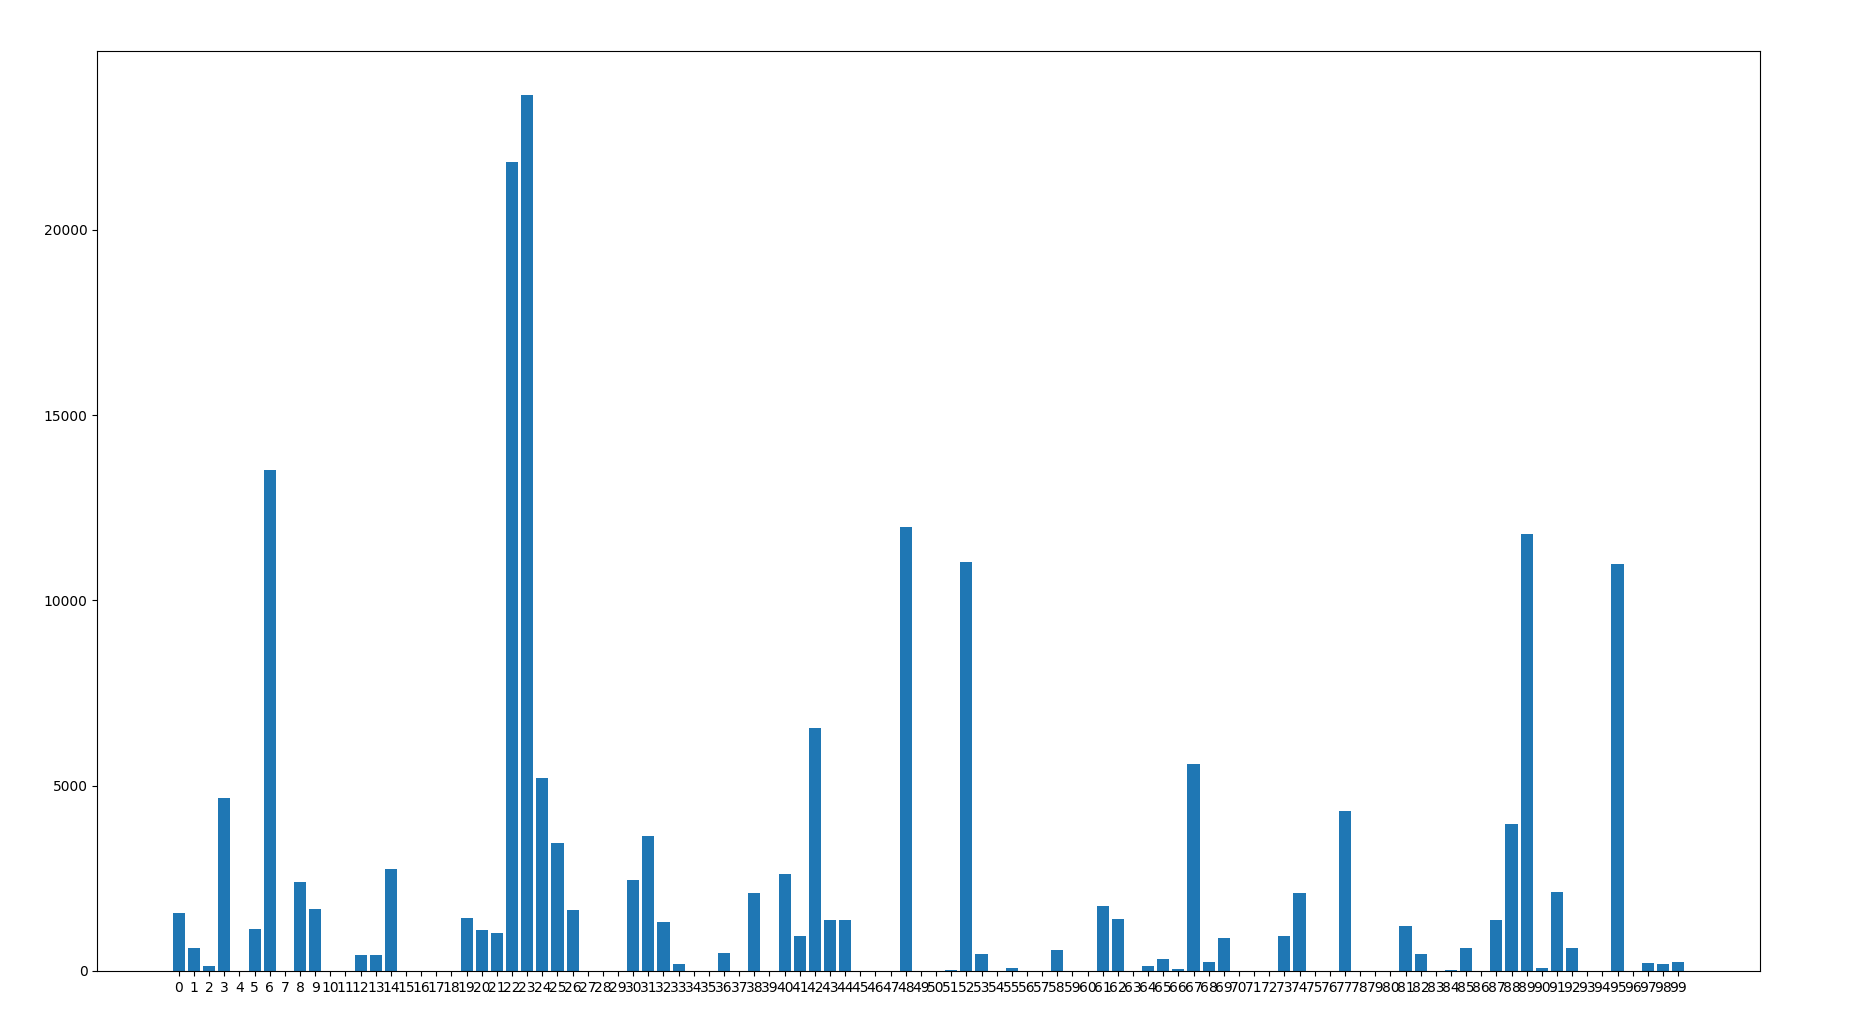
\includegraphics[width=\textwidth]{kitchen_hist}} \\
\end{tabular}
\caption{An image from kitchen class with its wordmap and corresponding histogram.}
\end{figure}

\subsection{Multi-resolution: Spatial Pyramid Matching}
Functions have been implemented and number of SPM layers chosen are 3.

\subsection{Comparing Images}
Functions have been implemented.

\subsection{Building A Model of the Visual World}
Functions have been implemented and \textit{trained\_system.npz} file has been created.

\subsection{Quantitative Evaluation}
The recognition system has been evaluated with the following metrics.

\begin{figure}[!ht]
\centering
\begin{BVerbatim}
[[ 7  0  0  0  5  4  3  1]
 [ 3 11  2  1  0  0  0  3]
 [ 1  2  9  0  2  1  2  3]
 [ 0  2  0 13  0  1  0  4]
 [ 6  0  0  1  7  3  1  2]
 [ 3  0  1  1  5  7  3  0]
 [ 0  1  0  1  1  3 14  0]
 [ 0  1  1  3  1  0  0 14]]
\end{BVerbatim}
\bigskip
\\
\textit{Confusion Matrix}
\end{figure}

\begin{equation*}
    Accuracy = 51.25\%
\end{equation*}

\begin{figure}[!ht]
    \centering
    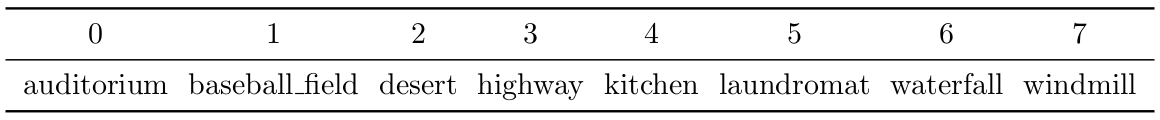
\includegraphics[width=\textwidth]{labels}
\end{figure}

\subsection{Find the Failed Cases}
From the confusion matrix above, the following can be inferred.
\begin{itemize}
    \item The classes \textit{auditorium}, \textit{kitchen}, and \textit{laundromat} have been misclassified into each others categories more often comparatively. This is probably because a lot of the objects and features are common to these classes.
    \item A similar observation can be made with the classes \textit{highway} and \textit{windmill} with few images misclassified, again probably because both of these classes have roads common in them.
    \item The \textit{desert} class has been classified incorrectly and is distributed between various classes. The reason could be that, this class has very few features and uniform regions, and hence being represented by fewer visual words, and consequently fewer features for the recognition system to distinguish it from the other classes well. 
    \item The classes \textit{waterfall} and \textit{windmill} have the best prediction accuracy with 70\% each and the reason for this is that they have some unique features such as water and the windmill blades which are not common to the other classes.
\end{itemize}

\section{Deep Learning Features - An Alternative to “Bag of Words”}
\subsection{Extracting Deep Features}
The various operations have been implemented and the forward pass through all the layers for a single image takes around 50-60 seconds. The custom implementation has also been verified with PyTorch implementation of VGG-16 and the results at the \textit{fc7} layer have been compared and they match (used \texttt{numpy.allclose}). The following function has been written to compare and verify the results.

\begin{figure}[!ht]
\centering
\begin{BVerbatim}
deep_recog.evaluate_custom_implementation()
\end{BVerbatim}
\end{figure}

\subsection{Building a Visual Recognition System: Revisited}
\begin{figure}[!ht]
\centering
\begin{BVerbatim}
[[20  0  0  0  0  0  0  0]
 [ 1 17  1  0  0  0  1  0]
 [ 0  0 18  2  0  0  0  0]
 [ 0  0  0 20  0  0  0  0]
 [ 0  0  0  0 18  2  0  0]
 [ 0  0  0  0  2 18  0  0]
 [ 0  0  0  0  0  0 20  0]
 [ 0  0  1  1  0  0  0 18]]
\end{BVerbatim}
\bigskip
\\
\textit{Confusion Matrix}
\end{figure}

\begin{equation*}
    Accuracy = 93.125\%
\end{equation*}

\begin{figure}[!ht]
    \centering
    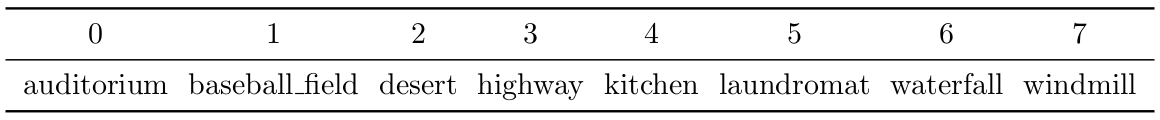
\includegraphics[width=\textwidth]{labels}
\end{figure}

The classification results using VGG-16 features are definitely better than using Spatial Pyramid Matching. Some of the reasons are listed below.
\begin{itemize}
    \item One of the main reasons is that we used only 3 layers in SPM which lead to a significant loss of spatial information. By increasing the number of layers in SPM, we can expect better accuracy with Bag of Words.  
    \item We used a filter bank of size 20 in BoW, which is very less compared to the number of filters that VGG-16 extracts. The type of features extracted in BoW just included horizontal/vertical edges, LoG and Gaussian filters, it did not even have a set of oriented edge detection filters. However, on visualizing some of the output responses of the initial \textit{conv2d} layers of VGG-16, it did have a lot of responses that extracted oriented edges as well. This definitely helps in classifying the images and overcome some of the problems discussed earlier with BoW.
    \item The \textit{maxpool} layers in the VGG-16 model, help in reducing the spatial dimension by retaining only the most important information. However, at the same time, they do not discard the spatial information significantly. This also makes the classification somewhat invariant to rotation, while classifying the test images.
    \item Another reason could be that the weights that VGG-16 uses have been trained with around 14 million images compared the feature extraction of BoW with just 1,440 images.
\end{itemize}

\end{document}